\chapter{Measurements and Evaluation}

\section{Initial Test Setup}
In order to evaluate the performance increase obtained when using a dedicated
hashing accelerator, a system-on-chip test system was constructed using Xilinx' Vivado
development studio, version 2014.3.

\begin{sidewaysfigure}[ht]
	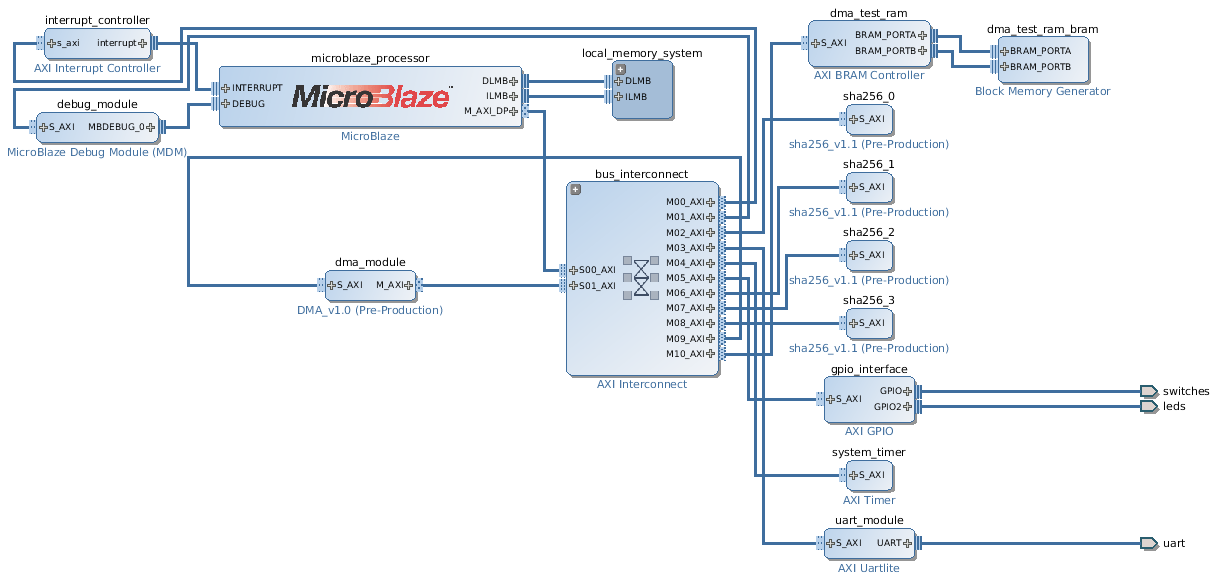
\includegraphics[width=0.95\textwidth]{Figures/testsystem-vivado.png}
	\caption{Overview of the initial test system}
	\label{fig:testsystem-vivado}
\end{sidewaysfigure}

The test system is controlled by a MicroBlaze microprocessor, configured to
include the optional barrel shifter, integer divider and pattern comparator extensions.
In order to run the XilKernel real-time operating system, the system also
includes a simple timer module for use by the kernel.

A UartLite module was included to provide I/O in order to communicate with
the system from a desktop computer, as well as a GPIO module for additional
debugging use.

The system runs on a 50~MHz clock which is synthesized by a clock generator
module from a 100~MHz input clock.

In order to run performance tests on the system, the DMA described in
section \ref{sec:dma-architecture} and four
SHA256 hashing modules are included.
A fixed-interval timer, that generates an interrupt every second, is
included in order to calculate the performance per second.

\subsection{Test Software}
In order to test the hashing modules and how the performance scales when including
additional hashing modules, a benchmark application was written. The benchmark
runs a specified number of threads that tries to hash a single block of data
over and over again.

A simple scheduler is used to provide each thread with an available hashing module.
If no module is available, the thread blocks on a semaphore until a module is available.

Once a second, the number of completed hashes for each module is added up and
reported over the UART.

The test software is also designed so that it can be run with a software implementation
of the hashing algorithm instead of the hashing modules. This makes it possible
to compare the performance when using an accelerator as compared to not using
an accelerator.\todo{Update test software description.}

\subsection{Measurements and Benchmarks}
The most important performance measure for a Bitcoin mining system is the number
of hashes per second it can sustain. Therefore, once a second the number of hashes
computed since the previous second is calculated and sent over the UART.

Another important measurement is how the inclusion of a DMA affects the performance
of the system.

\section{Revised Test System}

During the initial round of testing, it was discovered that using multiple hashing
modules did not increase the amount of hashes performed per second. The number remained
constant, while the total amount of hashing work was divided evenly between
the hashing modules. The maximum performance attained did not exceed 15~100~H/s.
It was discovered that the reason for this was that the bus system used did not have
enough bandwidth to sustain a higher amount of performance. Alternative bus topologies
could be used to alleviate this issue, but is left for future work and described in
section \ref{sec:future-work}.

Since using multiple hashing modules would not provide any benefit, they were removed
from the test system to simplify testing. In addition, removing the extraneous modules
made it possible to make the test software single-threaded, removing any overhead from
using the XilKernel for multi-threading.

The revised test system is illustrated in figure \ref{fig:testsystem-vivado-final}.

\begin{sidewaysfigure}[ht]
	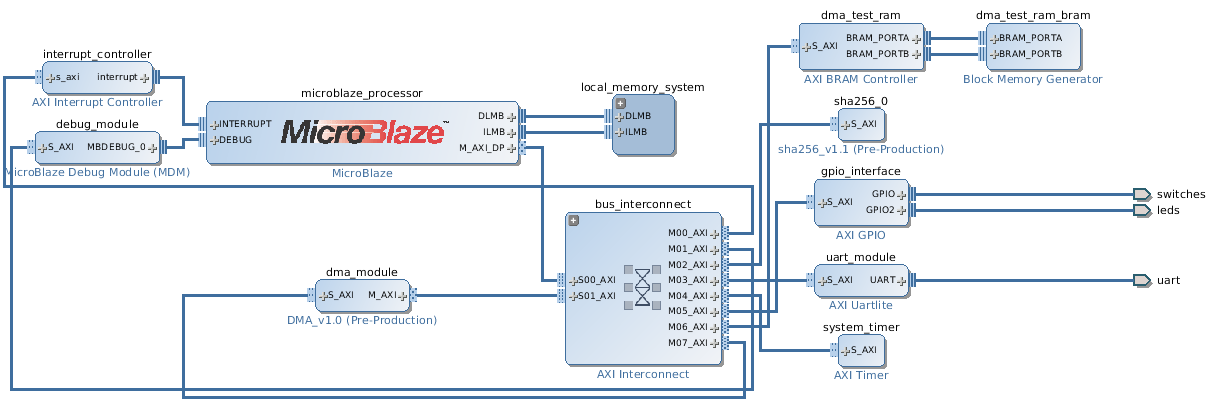
\includegraphics[width=0.95\textwidth]{Figures/testsystem-vivado-final.png}
	\caption{Overview of the final test system}
	\label{fig:testsystem-vivado-final}
\end{sidewaysfigure}

\section{Results}

Using the revised test system, three measurements were made in order to evaluate the
performance of the hashing accelerator. The number of hashes per second were measured
both when using a DMA for data transfer between RAM and the hashing tile and when not
using a DMA. The results are compared to a software implementation of the algorithm
running on the MCU.

\begin{table}[ht]
	\centering
	\begin{tabular}{|l|l|}
		\hline
		\textbf{Methodology} & \textbf{Result} \\
		\hline
		Software & 849~H/s \\
		Hardware without DMA & 16~196~H/s\\
		Hardware with DMA & 12~240~H/s\\
		\hline
	\end{tabular}

	\caption{Test results}
\end{table}

\section{Evaluation}

The results clearly shows the benefit of using a hashing module over doing hashing in software,
obtaining a speedup of 19 times is over the software implementation.

However, using the DMA for data transfers causes a reduction in performance, although it is still
an improvement of 14,4 times over the software implementation. The reason for this is that the
DMA module was initially designed to work with a word addressed bus system, increasing the
address by 1 word for each bus request. This resulted in four requests per 32-bit word in
the test system, which caused the reduction in performance.

However, the speed-up when using no DMA as compared to using the DMA to transfer data is only
1,3 times, which is not enough to discourage use of the DMA even when the DMA does more transfers
than neccessary. Since the CPU can sleep or work on other tasks, using the inefficient DMA may
still be more energy efficient than not using a DMA at all.

It is expected that using a DMA with proper addressing will increase the performance obtained
with the DMA over the performance obtained without the DMA; assuming the bus is the bottleneck,
a DMA which uses proper addressing will issue only 1 request per word instead of 4, causing
less buss congestion and higher performance, possibly increasing the performance by up to
four times.

